%%%%%%%%%%%%%%%%%%%%%%%%%%%%%%%%%%%%%%%%%
% Beamer Presentation
% LaTeX Template
% Version 1.0 (10/11/12)
%
% This template has been downloaded from:
% http://www.LaTeXTemplates.com
%
% License:
% CC BY-NC-SA 3.0 (http://creativecommons.org/licenses/by-nc-sa/3.0/)
%
%%%%%%%%%%%%%%%%%%%%%%%%%%%%%%%%%%%%%%%%%

%----------------------------------------------------------------------------------------
% PACKAGES AND THEMES
%----------------------------------------------------------------------------------------

\documentclass{beamer}

\mode<presentation> {

% The Beamer class comes with a number of default slide themes
% which change the colors and layouts of slides. Below this is a list
% of all the themes, uncomment each in turn to see what they look like.

%\usetheme{default}
%\usetheme{AnnArbor}
%\usetheme{Antibes}
%\usetheme{Bergen}
%\usetheme{Berkeley}
%\usetheme{Berlin}
%\usetheme{Boadilla}
%\usetheme{CambridgeUS}
%\usetheme{Copenhagen}
%\usetheme{Darmstadt}
%\usetheme{Dresden}
%\usetheme{Frankfurt}
%\usetheme{Goettingen}
%\usetheme{Hannover}
%\usetheme{Ilmenau}
%\usetheme{JuanLesPins}
%\usetheme{Luebeck}
\usetheme{Madrid}
%\usetheme{Malmoe}
%\usetheme{Marburg}
%\usetheme{Montpellier}
%\usetheme{PaloAlto}
%\usetheme{Pittsburgh}
%\usetheme{Rochester}
%\usetheme{Singapore}
%\usetheme{Szeged}
%\usetheme{Warsaw}

% As well as themes, the Beamer class has a number of color themes
% for any slide theme. Uncomment each of these in turn to see how it
% changes the colors of your current slide theme.

%\usecolortheme{albatross}
%\usecolortheme{beaver}
%\usecolortheme{beetle}
%\usecolortheme{crane}
%\usecolortheme{dolphin}
%\usecolortheme{dove}
%\usecolortheme{fly}
%\usecolortheme{lily}
%\usecolortheme{orchid}
%\usecolortheme{rose}
%\usecolortheme{seagull}
%\usecolortheme{seahorse}
%\usecolortheme{whale}
%\usecolortheme{wolverine}

%\setbeamertemplate{footline} % To remove the footer line in all slides uncomment this line
%\setbeamertemplate{footline}[page number] % To replace the footer line in all slides with a simple slide count uncomment this line

%\setbeamertemplate{navigation symbols}{} % To remove the navigation symbols from the bottom of all slides uncomment this line
}

\usepackage{graphicx} % Allows including images
\usepackage{booktabs} % Allows the use of \toprule, \midrule and \bottomrule in tables

%----------------------------------------------------------------------------------------
% TITLE PAGE
%----------------------------------------------------------------------------------------

\title[Breadboard to PCB]{Open Hardware: Breadboard to PCB} % The short title appears at the bottom of every slide, the full title is only on the title page

\author{Jenner Hanni} % Your name
\institute[Open Source Bridge 2014] % Your institution as it will appear on the bottom of every slide, may be shorthand to save space
{
Open Source Bridge 2014 \\ % Your institution for the title page
\medskip
\textit{jeh.wicker@gmail.com} 
}

\begin{document}

\begin{frame}
\titlepage % Print the title page as the first slide
\end{frame}

\begin{frame}
\frametitle{Overview} % Table of contents slide, comment this block out to remove it
\tableofcontents % Throughout your presentation, if you choose to use \section{} and \subsection{} commands, these will automatically be printed on this slide as an overview of your presentation
\end{frame}

%----------------------------------------------------------------------------------------
% PRESENTATION SLIDES
%----------------------------------------------------------------------------------------

%------------------------------------------------
\section{Oven Controller Project} 
%------------------------------------------------
\subsection{Background}
%------------------------------------------------
\begin{frame}
\frametitle{Portland State Aerospace Society}
\begin{figure}
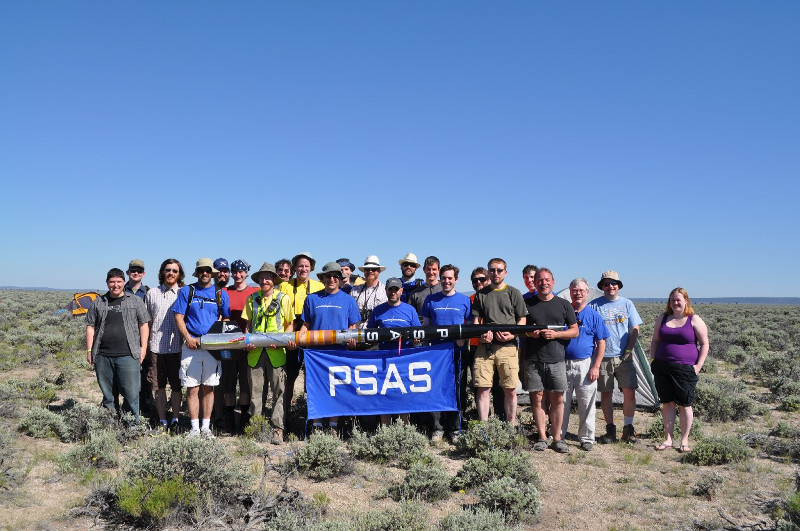
\includegraphics[width=0.9\linewidth]{psas.jpg}
\end{figure}
\end{frame}
%------------------------------------------------
\begin{frame}
\frametitle{"We built you an oven!"}
\begin{figure}
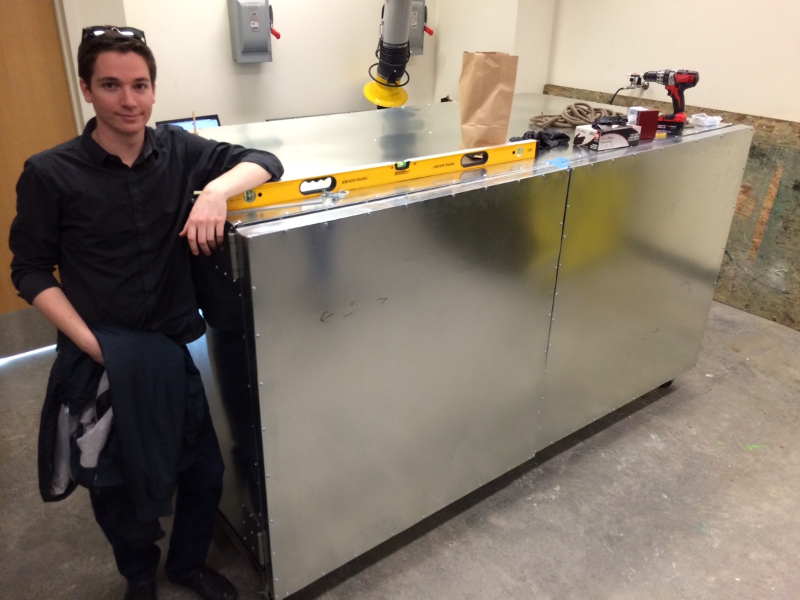
\includegraphics[width=0.8\linewidth]{curing-oven.png}
\end{figure}
\end{frame}
%------------------------------------------------
\begin{frame}
\frametitle{"... here are the electronics!"}
\begin{figure}
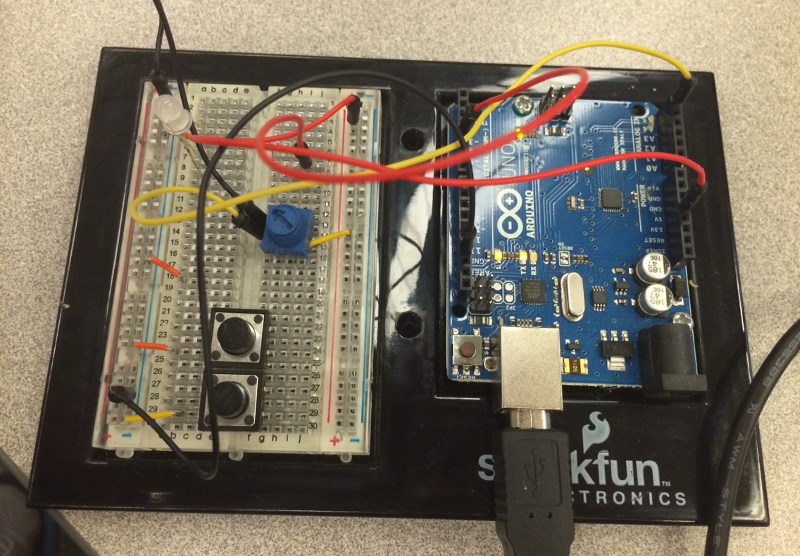
\includegraphics[width=0.9\linewidth]{breadboard.png}
\end{figure}
\end{frame}
%------------------------------------------------
\begin{frame}
\frametitle{Through-hole Arduino Shield}
\begin{figure}
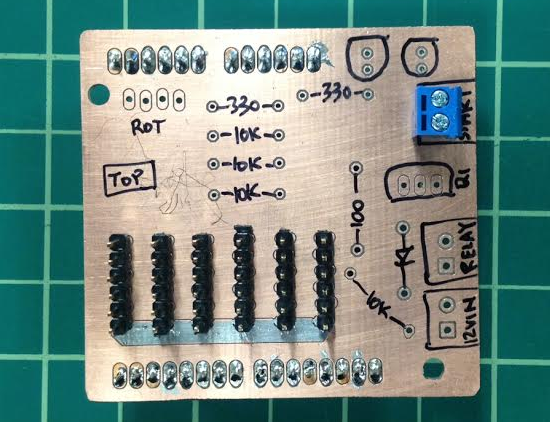
\includegraphics[width=0.9\linewidth]{ovenboard-top.png}
\end{figure}
\end{frame}
%------------------------------------------------
\begin{frame}
\frametitle{Surface-mount Arduino Shield}
\begin{figure}
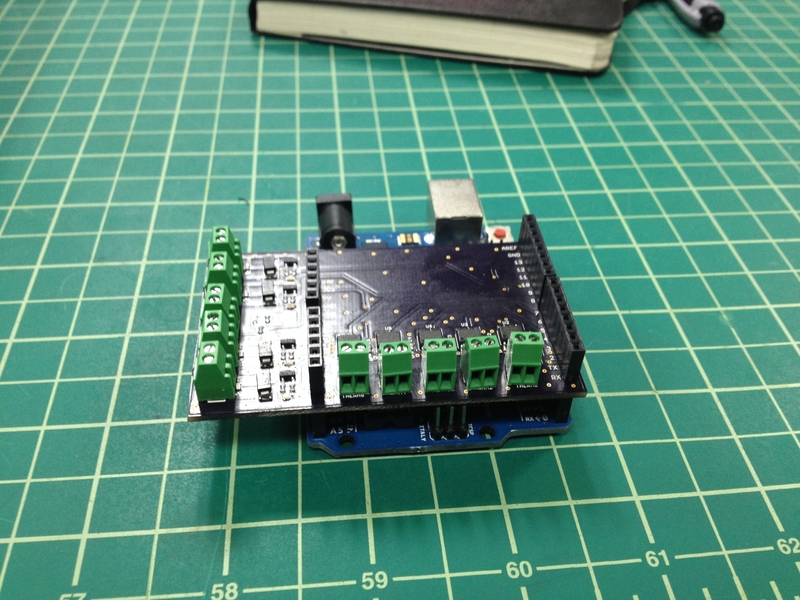
\includegraphics[width=0.9\linewidth]{ovenboard3-side.png}
\end{figure}
\end{frame}
%------------------------------------------------
\begin{frame}
\frametitle{Finished product}
\begin{figure}
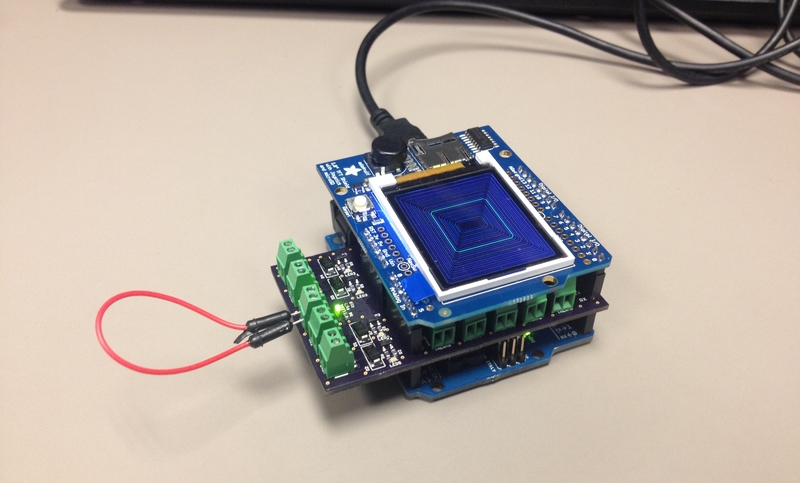
\includegraphics[width=0.9\linewidth]{ovenboard3-final.png}
\end{figure}
\end{frame}


%------------------------------------------------
\subsection{Terminology}

\begin{frame}
\Huge{\centerline{Terminology}}
\end{frame}

%------------------------------------------------

\begin{frame}
\frametitle{Layer Stackup}

\begin{figure}
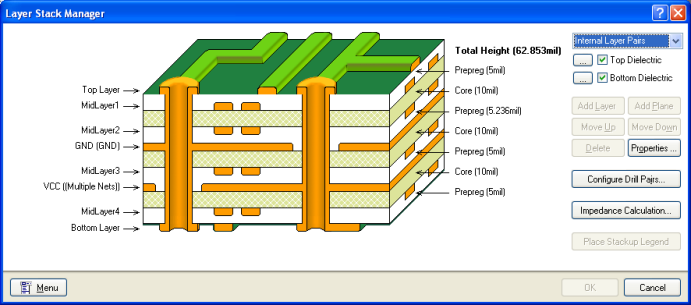
\includegraphics[width=0.8\linewidth]{stackup.png}
\end{figure}

\end{frame}

%------------------------------------------------
\begin{frame}
\frametitle{Vias}
\begin{columns}[c] % The "c" option specifies centered vertical alignment while the "t" option is used for top vertical alignment

\column{.45\textwidth} % Left column and width
\begin{enumerate}
\item Through-hole
\item Blind
\item Buried
\end{enumerate}

\column{.5\textwidth} % Right column and width
\begin{figure}
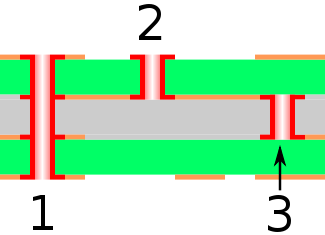
\includegraphics[width=0.8\linewidth]{vias.png}
\end{figure}

\end{columns}
\end{frame}

%------------------------------------------------

\begin{frame}
\frametitle{Soldermask}
\begin{figure}
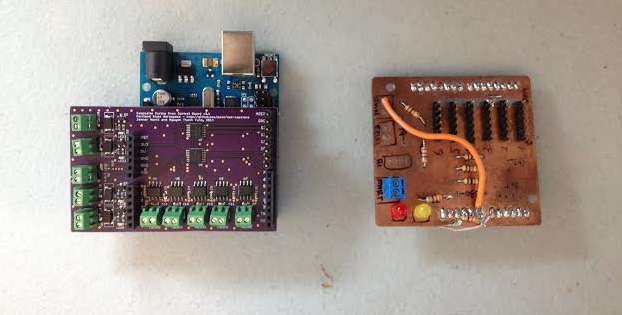
\includegraphics[width=1\linewidth]{soldermask.png}
\end{figure}
\end{frame}

%------------------------------------------------

\begin{frame}
\frametitle{Reflow}
\begin{columns}[c] % The "c" option specifies centered vertical alignment while the "t" option is used for top vertical alignment

\column{.45\textwidth} % Right column and width
\textbf{Reflow Profile}
\begin{enumerate}
\item Leaded
\item Non-leaded
\end{enumerate}

\column{.45\textwidth} % Right column and width
\begin{figure}
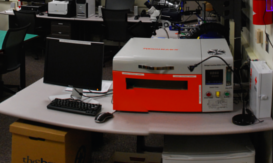
\includegraphics[width=0.8\linewidth]{psu-epl.png}
\end{figure}

\end{columns}
\end{frame}

%------------------------------------------------
\begin{frame}
\Huge{\centerline{Let's make a printed circuit board.}}
\end{frame}
%------------------------------------------------

\begin{frame}
\frametitle{Process}

\begin{enumerate}
\item Make decisions
\item Choose parts
\item Draw schematic
\item Draw layout
\item Buy parts
\item Fab the board
\item Assemble the board
\item Test the board
\end{enumerate}

\end{frame}

%------------------------------------------------
\section{Making Decisions} 
\subsection{Parts, Design Tool, Fab, Assembly} 
\begin{frame}
\Huge{\centerline{Making Decisions}}
\end{frame}
%------------------------------------------------

\begin{frame}
\frametitle{Making Decisions: Parts and Assembly}
\begin{columns}[t] % The "c" option specifies centered vertical alignment while the "t" option is used for top vertical alignment

\column{.45\textwidth} % Right column and width
\centerline{\textbf{Through-hole}}
\begin{figure}
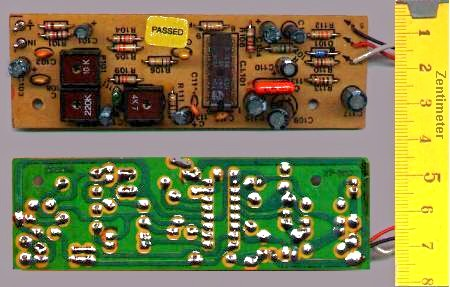
\includegraphics[width=0.8\linewidth]{th.jpg}
\end{figure}
\centerline{Solder by hand}

\column{.45\textwidth} % Right column and width
\centerline{\textbf{Surface-mount}}
\begin{figure}
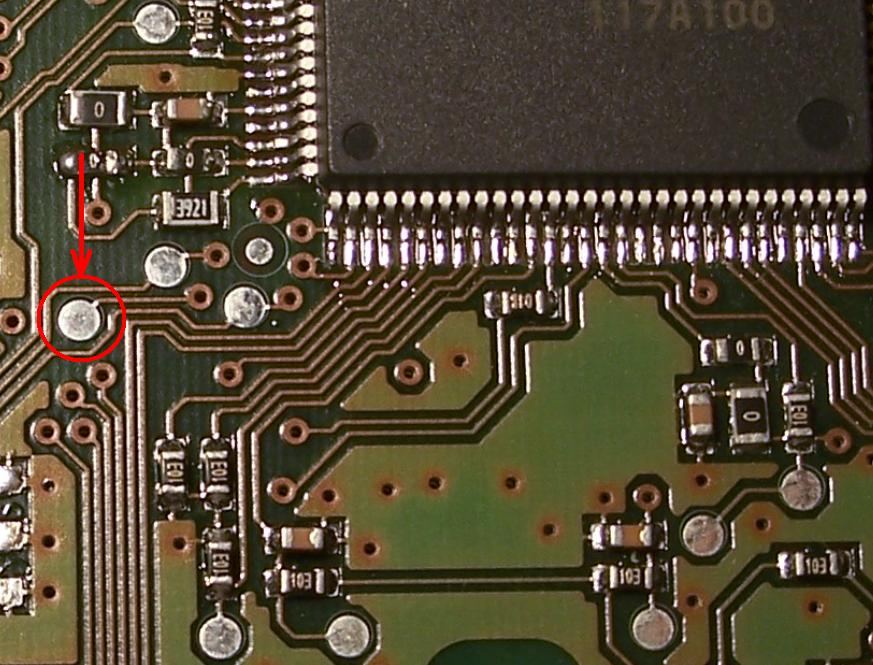
\includegraphics[width=0.8\linewidth]{smt.jpg}
\end{figure}
\centerline{Stencil, Reflow}

\end{columns}
\end{frame}

\begin{frame}
\frametitle{Making Decisions: Design Tool}
\begin{columns}[t] % The "c" option specifies centered vertical alignment while the "t" option is used for top vertical alignment

\column{.35\textwidth} % Right column and width
\begin{enumerate}
\item{Altium}
\item{DxDesigner/PADS}
\newline
\item{Eagle}
\newline
\item{gEDA}
\item{KiCad}
\end{enumerate}

\column{.65\textwidth} % Right column and width
\centerline{\textbf{KiCad}}
\begin{figure}
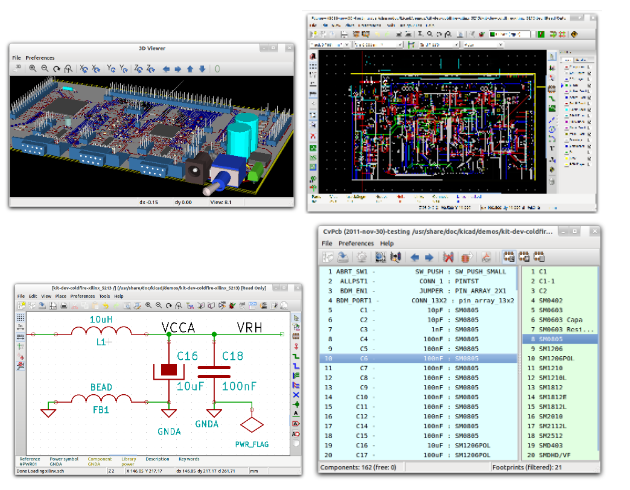
\includegraphics[width=0.8\linewidth]{kicad.png}
\end{figure}

\end{columns}
\end{frame}

\begin{frame}
\frametitle{Making Decisions: Fab House}
 
\begin{figure}
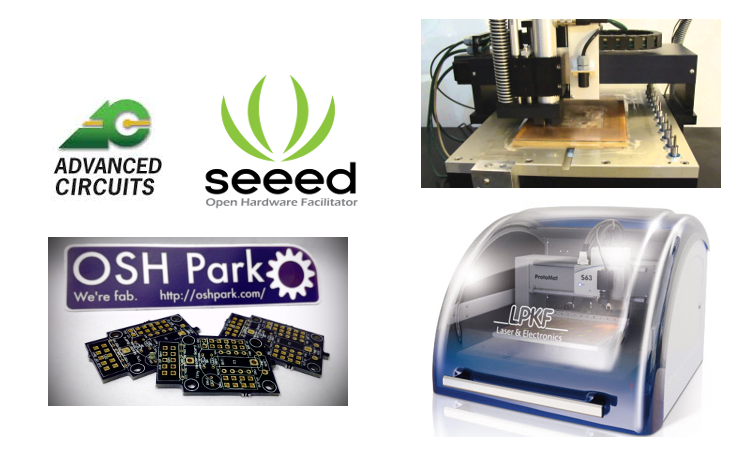
\includegraphics[width=0.9\linewidth]{fabs.png}
\end{figure}

\end{frame}

%------------------------------------------------
\section{PCB Design} 
\subsection{Through-hole}
\begin{frame}
\frametitle{Oven Board v1}
\begin{figure}
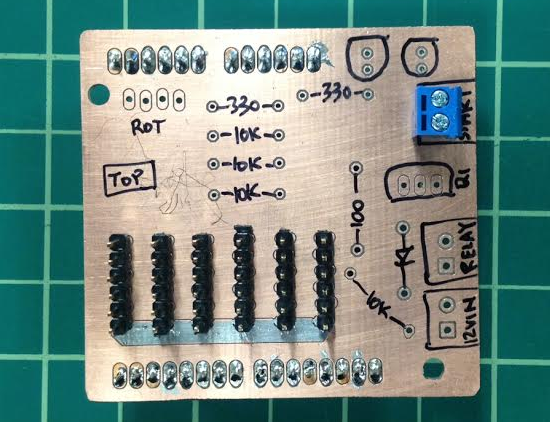
\includegraphics[width=0.8\linewidth]{ovenboard-top.png}
\end{figure}
\end{frame}
%------------------------------------------------------

\begin{frame}
\frametitle{v1 Decisions}
\begin{figure}
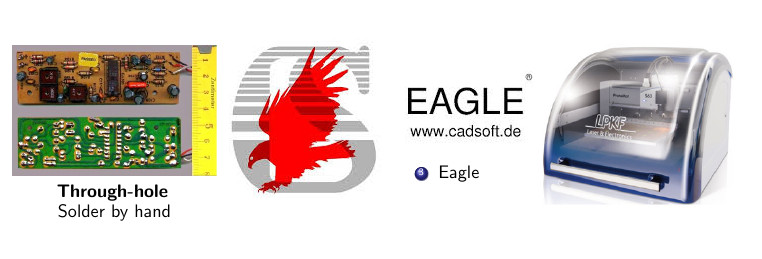
\includegraphics[width=1.0\linewidth]{decisions1.jpg}
\end{figure}
\end{frame}

%------------------------------------------------------

\begin{frame}
\frametitle{Grid}
0.001" = one thousandth of an inch = 1 mil != 1 millimeter
\begin{figure}
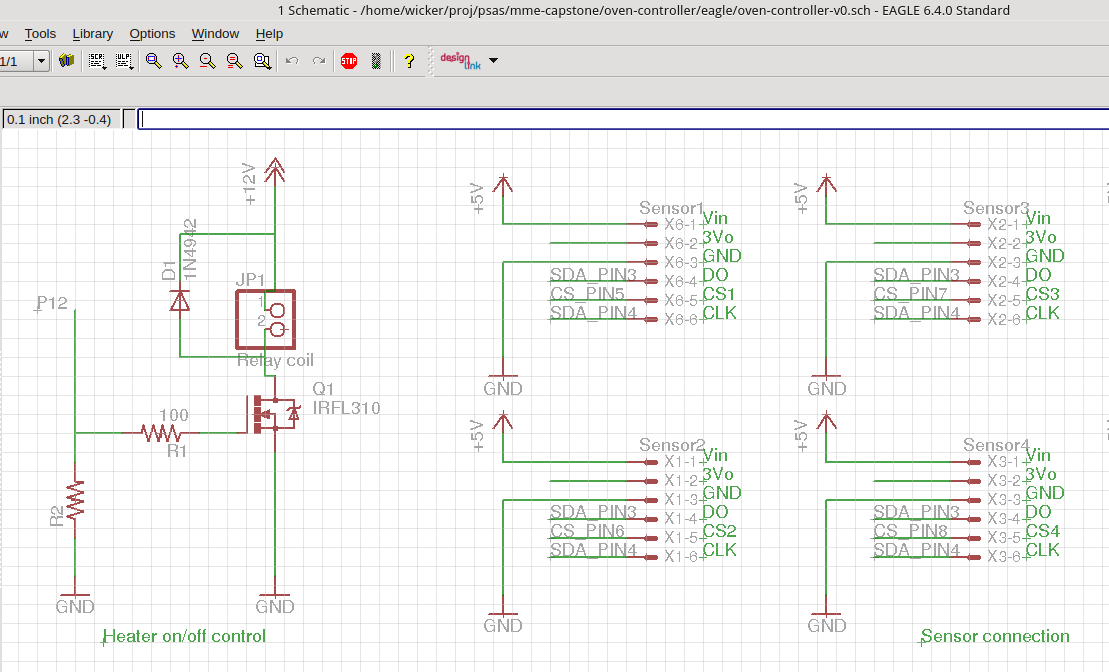
\includegraphics[width=1.0\linewidth]{grid.png}
\end{figure}
\end{frame}

%------------------------------------------------------

\begin{frame}
\frametitle{Place symbols with pins}
\begin{figure}
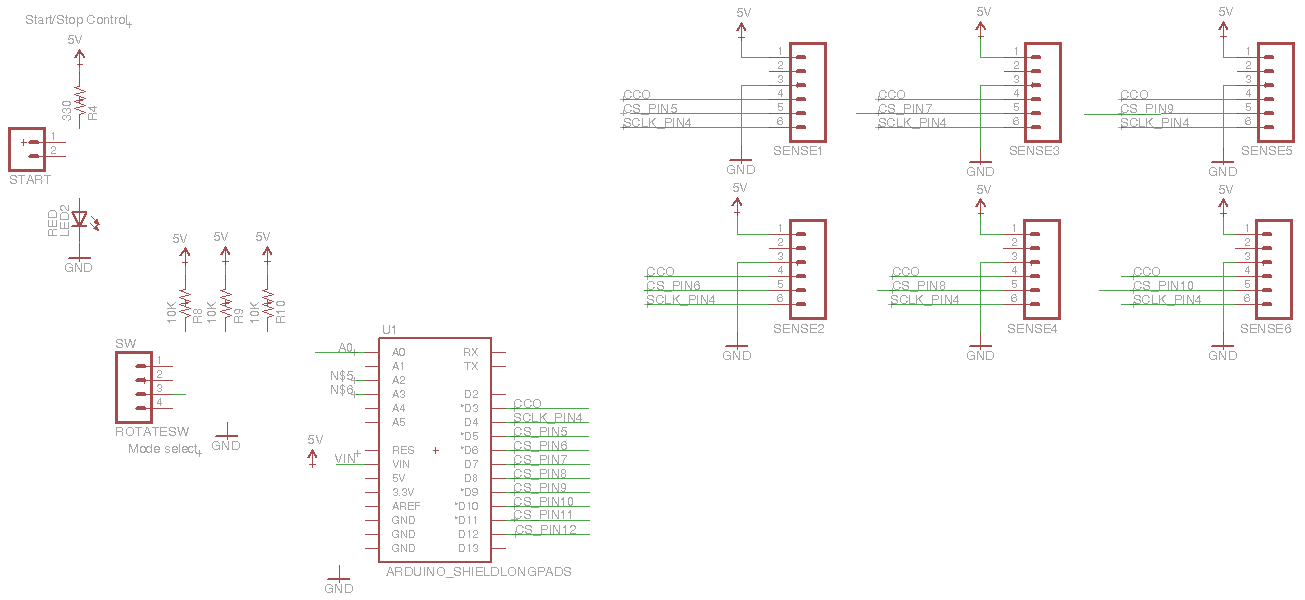
\includegraphics[width=1\linewidth]{symbols.png}
\end{figure}
\end{frame}

%------------------------------------------------------

\begin{frame}
\frametitle{Show connections!}
\begin{figure}
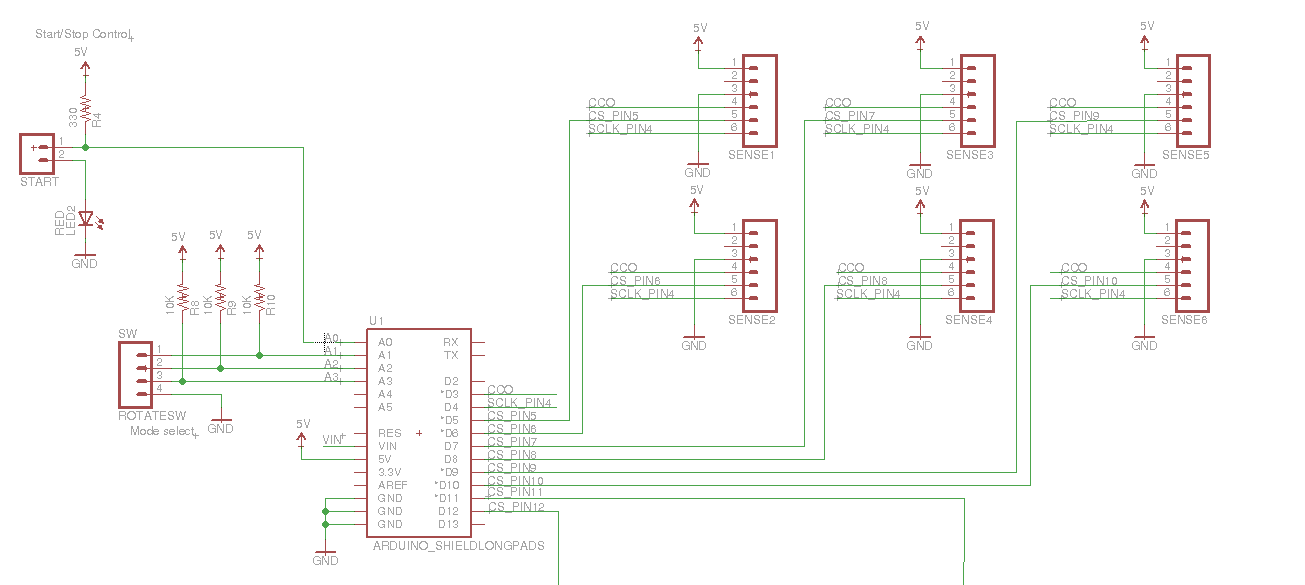
\includegraphics[width=1\linewidth]{symbols-connected.png}
\end{figure}
\end{frame}

%------------------------------------------------------

\begin{frame}
\frametitle{Things to think about}
\begin{enumerate}
\item Signal flow left to right
\item Power and ground
\item Symbol layout doesn't have to look like the footprint
\item Net names for traceability
\item Boxes around sections to show options or functionality
\item Multiple pages for a complicated circuit
\item Text to give more information - are you the layout person?
\end{enumerate} 
\end{frame}

%------------------------------------------------------

\begin{frame}
\frametitle{Bad Example: MAX2769 Eval Board}
\begin{figure}
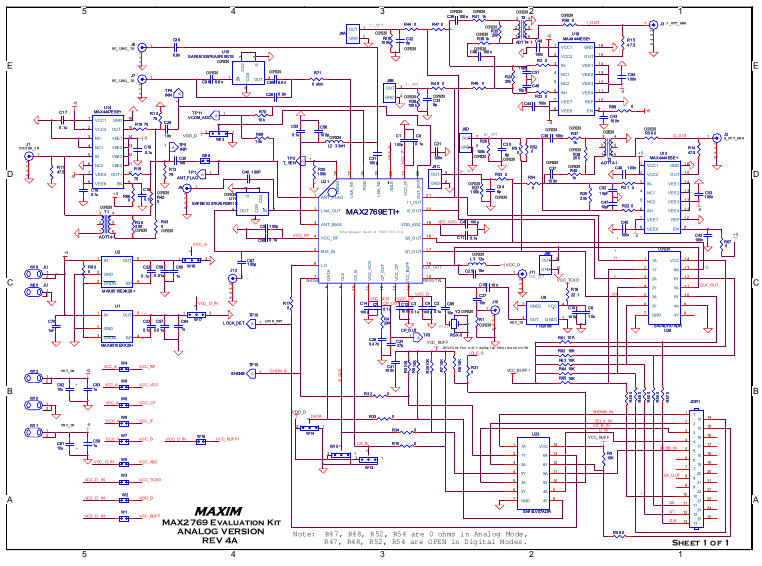
\includegraphics[width=0.9\linewidth]{badschema.png}
\end{figure}
\end{frame}

%------------------------------------------------------

\begin{frame}
\frametitle{Good Example: GPS RF Front-end Board}
\begin{figure}
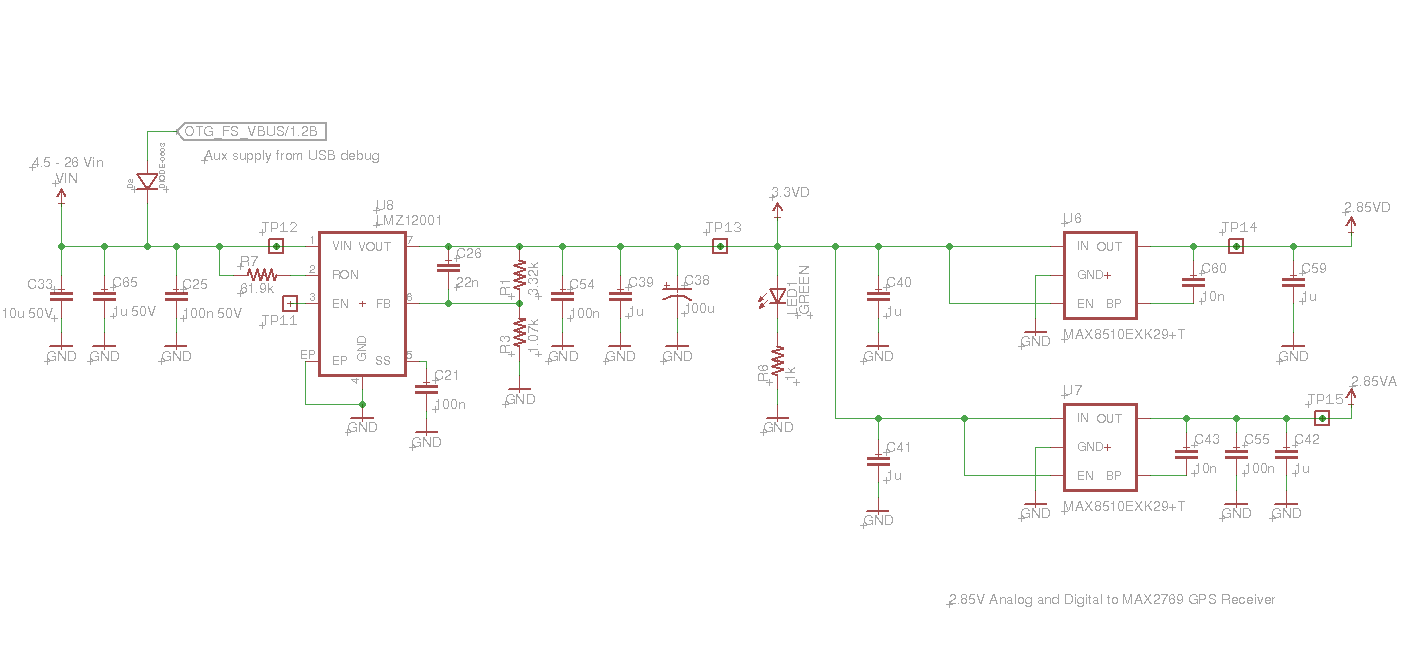
\includegraphics[width=1\linewidth]{schflow.png}
\end{figure}
\end{frame}

%------------------------------------------------------

\begin{frame}
\frametitle{Okay, now what?}
\begin{enumerate}
\item Design Review
\item Notebook
\item Remember, don't make this a waterfall process
\end{enumerate}
\end{frame}

%------------------------------------------------------

\begin{frame}
\frametitle{Board Layout}
\begin{figure}
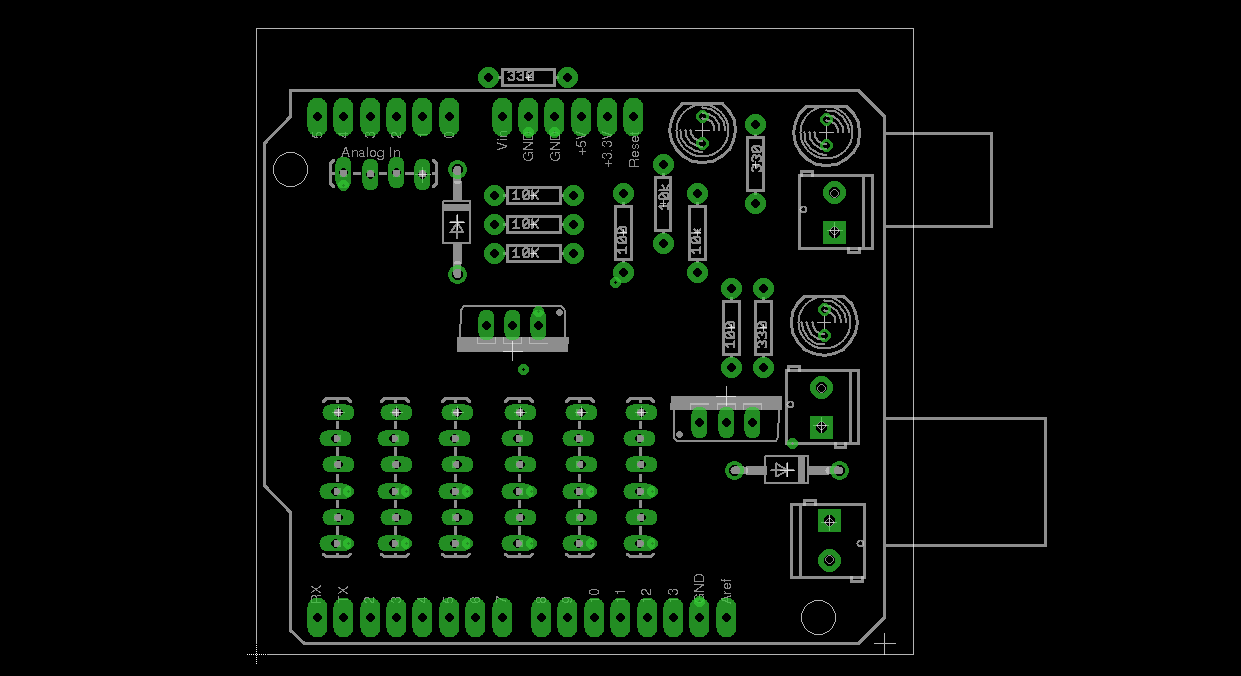
\includegraphics[width=1\linewidth]{boardnone.png}
\end{figure}
\end{frame}

%------------------------------------------------------

\begin{frame}
\frametitle{Board Layout}
\begin{figure}
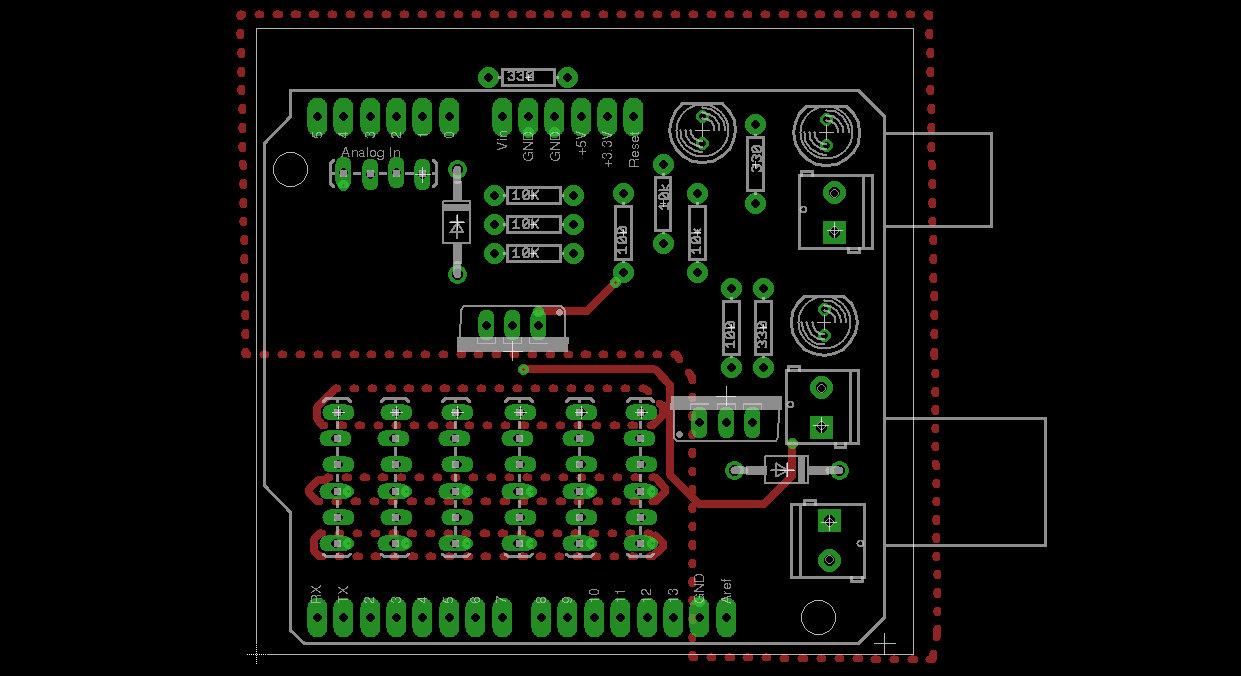
\includegraphics[width=1\linewidth]{boardtop.png}
\end{figure}
\end{frame}

%------------------------------------------------------

\begin{frame}
\frametitle{Board Layout}
\begin{figure}
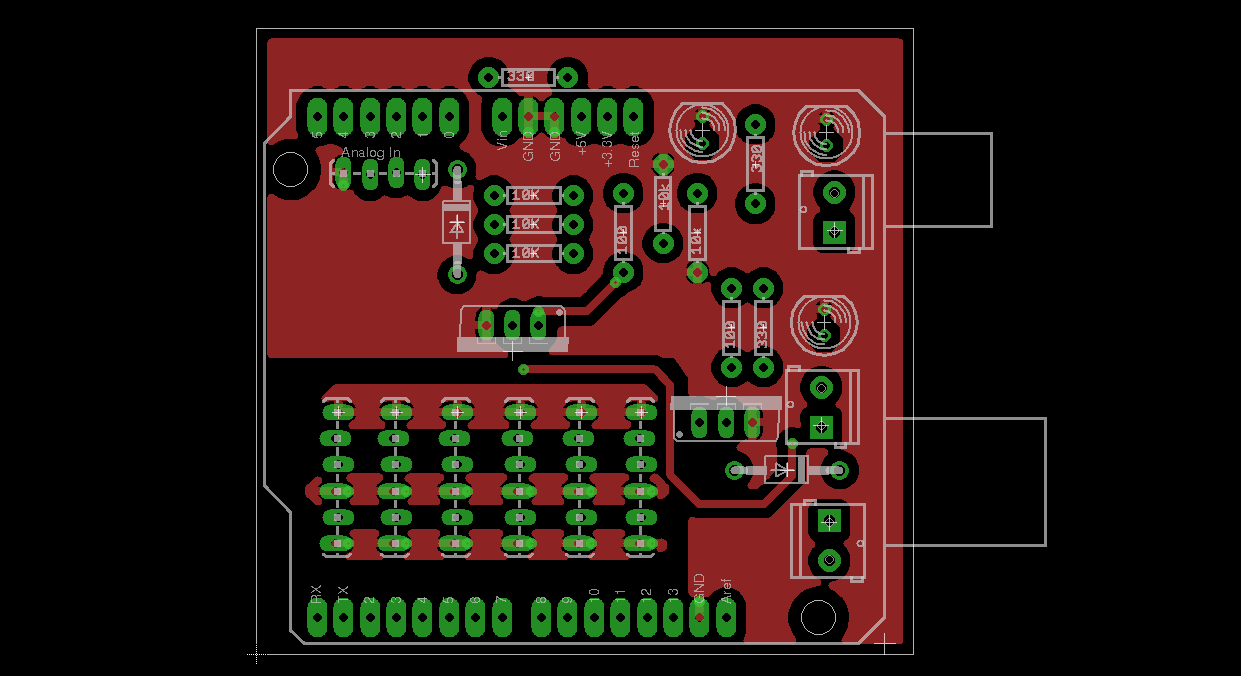
\includegraphics[width=1\linewidth]{boardfilltop.png}
\end{figure}
\end{frame}

%------------------------------------------------------

\begin{frame}
\frametitle{Board Layout}
\begin{figure}
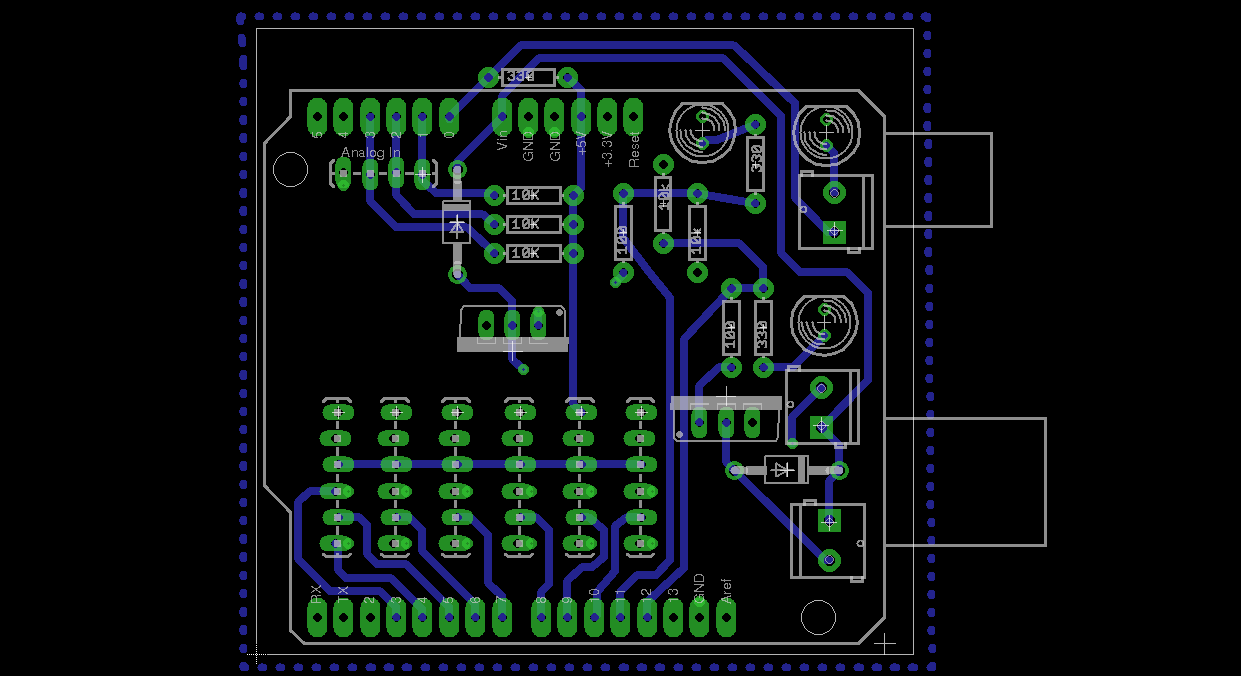
\includegraphics[width=1\linewidth]{boardbot.png}
\end{figure}
\end{frame}

%------------------------------------------------------

\begin{frame}
\frametitle{Board Layout}
\begin{figure}
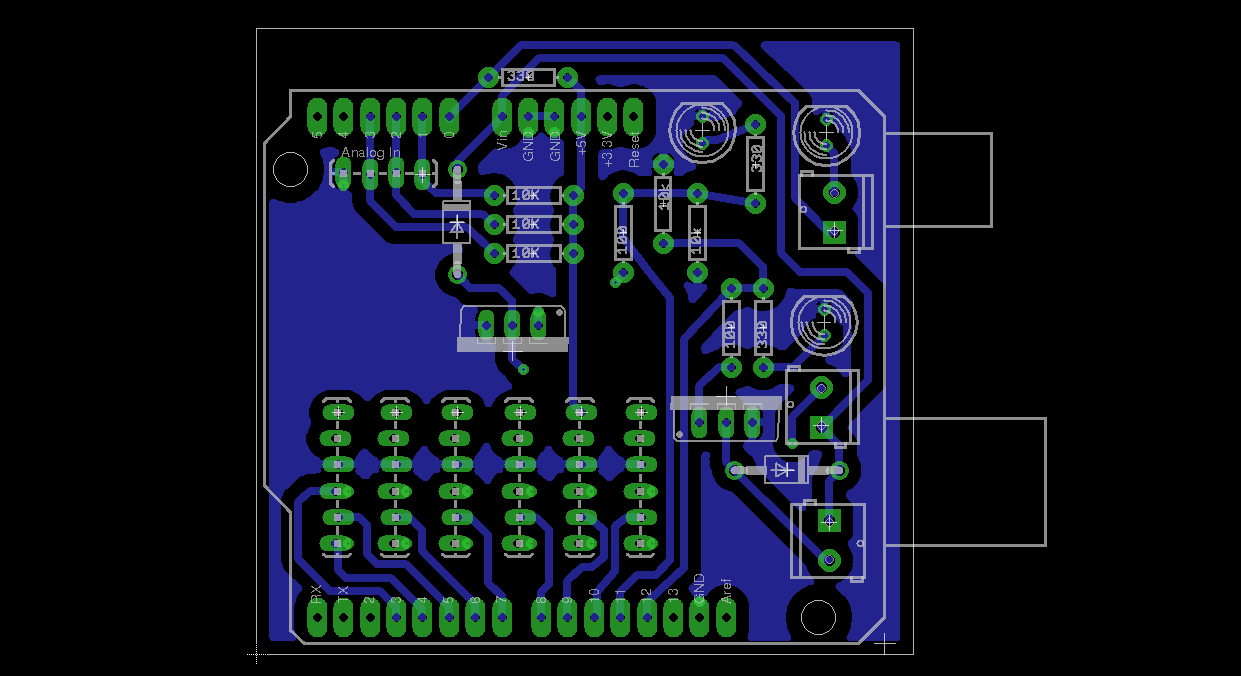
\includegraphics[width=1\linewidth]{boardfillbot.png}
\end{figure}
\end{frame}

%------------------------------------------------------

\begin{frame}
\frametitle{Board Layout}
\begin{figure}
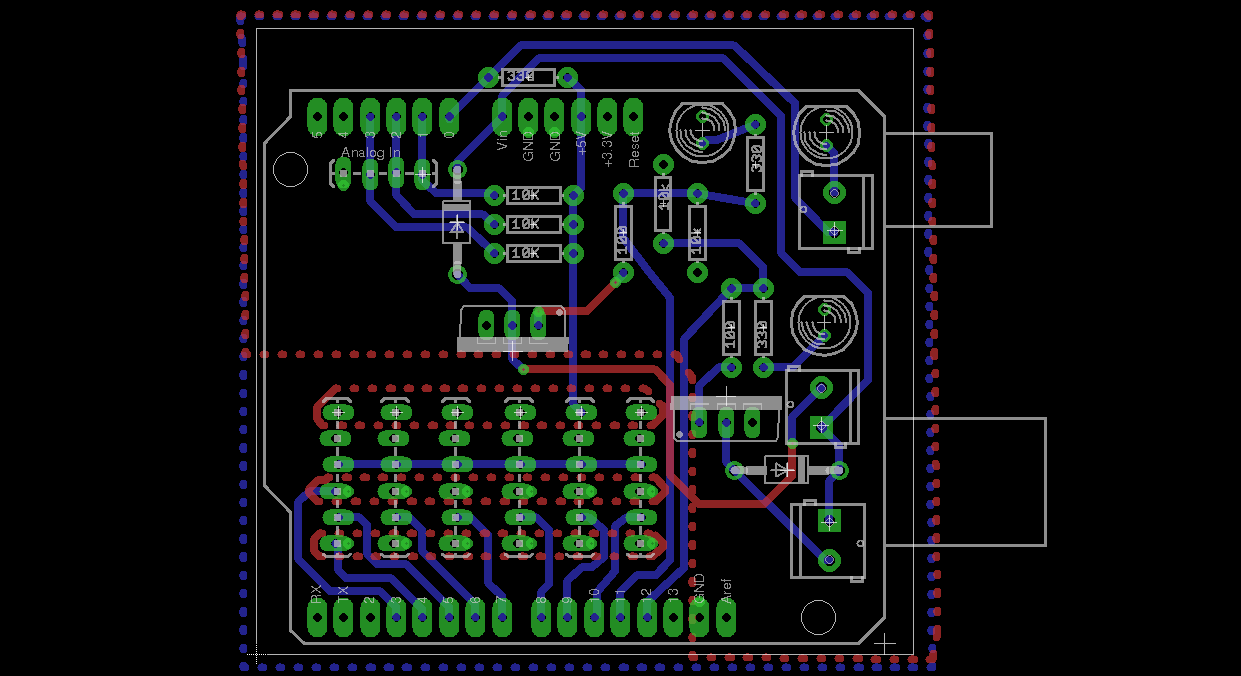
\includegraphics[width=1\linewidth]{boardall.png}
\end{figure}
\end{frame}

%------------------------------------------------------

\begin{frame}
\frametitle{Board Layout}
\begin{figure}
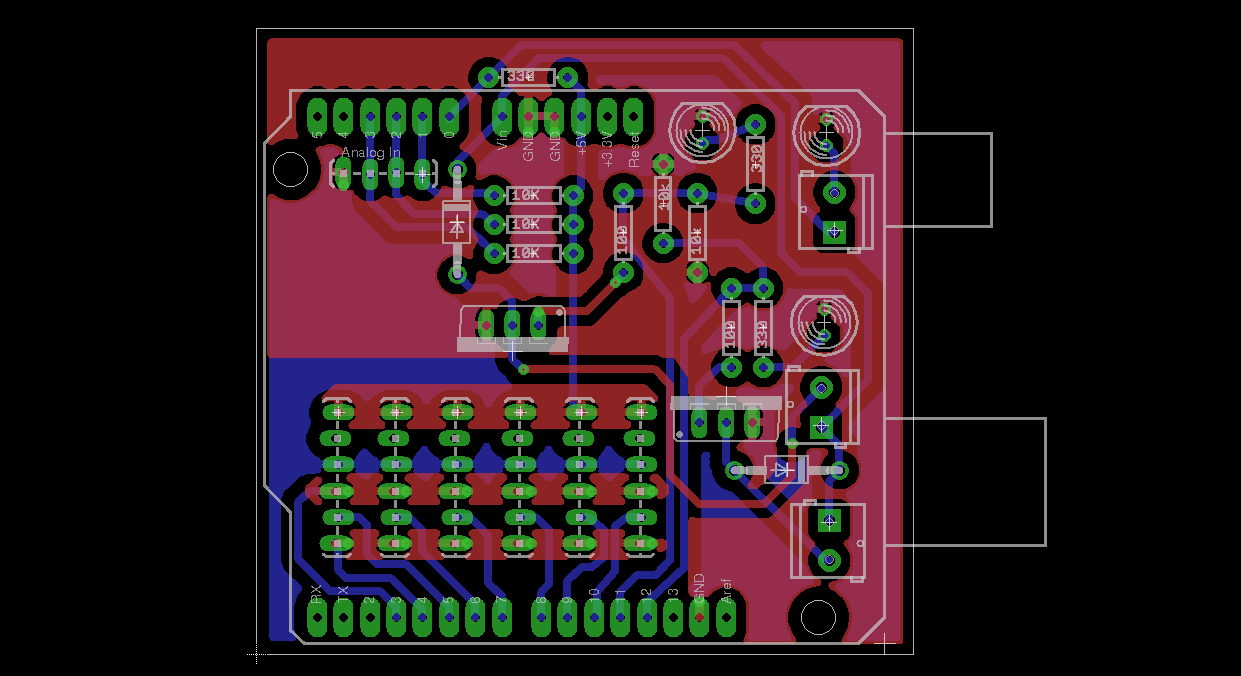
\includegraphics[width=1\linewidth]{boardfill.png}
\end{figure}
\end{frame}

%------------------------------------------------------

\begin{frame}
\frametitle{Gerbers}
Board Outline, Top, Bottom, Drills
\begin{figure}
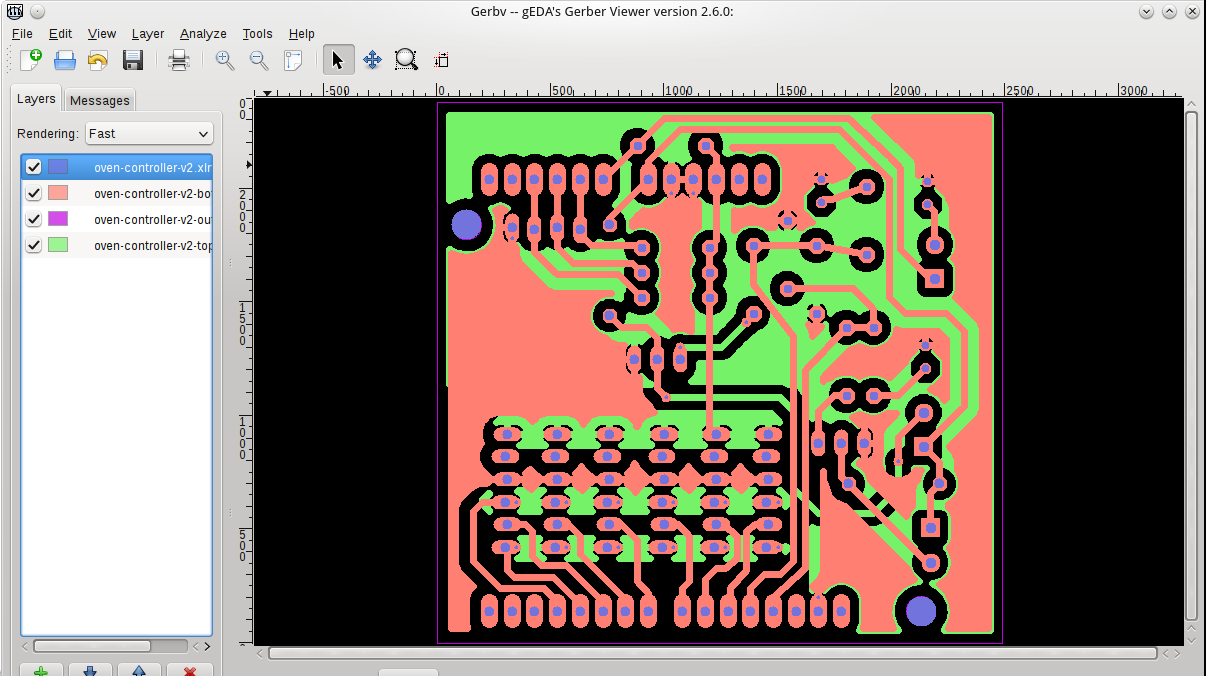
\includegraphics[width=1\linewidth]{gerbv.png}
\end{figure}
\end{frame}

%------------------------------------------------------

\begin{frame}
\frametitle{Fabricate with the LPKF}
\begin{figure}
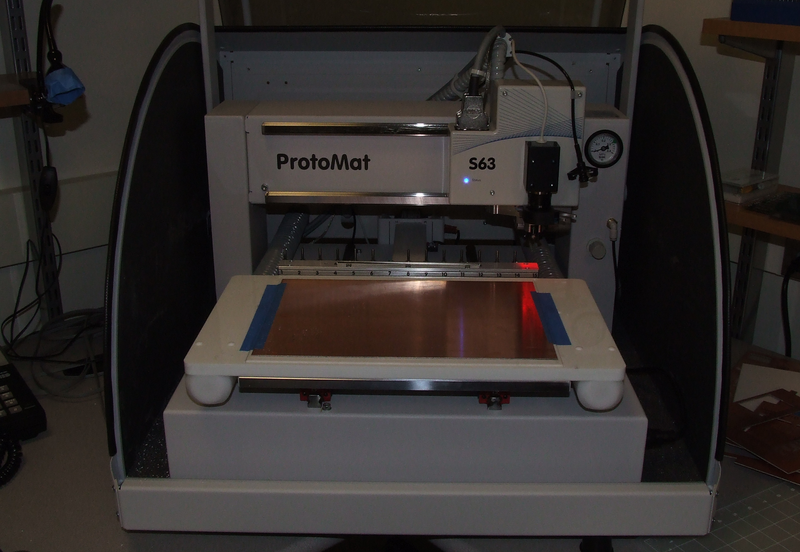
\includegraphics[width=1\linewidth]{fab-lpkf.png}
\end{figure}
\end{frame}

%------------------------------------------------------

\begin{frame}
\frametitle{Get the board back... now what?}
\begin{columns}[c] % The "c" option specifies centered vertical alignment while the "t" option is used for top vertical alignment

\column{.55\textwidth} % Right column and width
\begin{enumerate}
\item Inspect, test with a multimeter
\item Solder in parts
\item Test with a multimeter
\item Power it up
\end{enumerate}

\column{.3\textwidth} % Right column and width
\begin{figure}
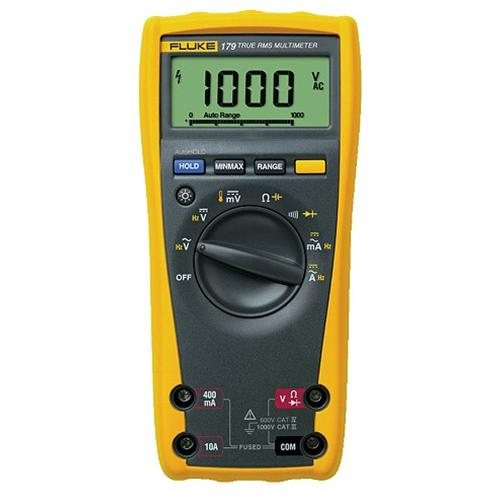
\includegraphics[width=0.8\linewidth]{fluke.jpg}
\end{figure}

\end{columns}
\end{frame}

%------------------------------------------------------
\subsection{Surface-mount}
\begin{frame}
\frametitle{Oven Board v3}
\begin{figure}
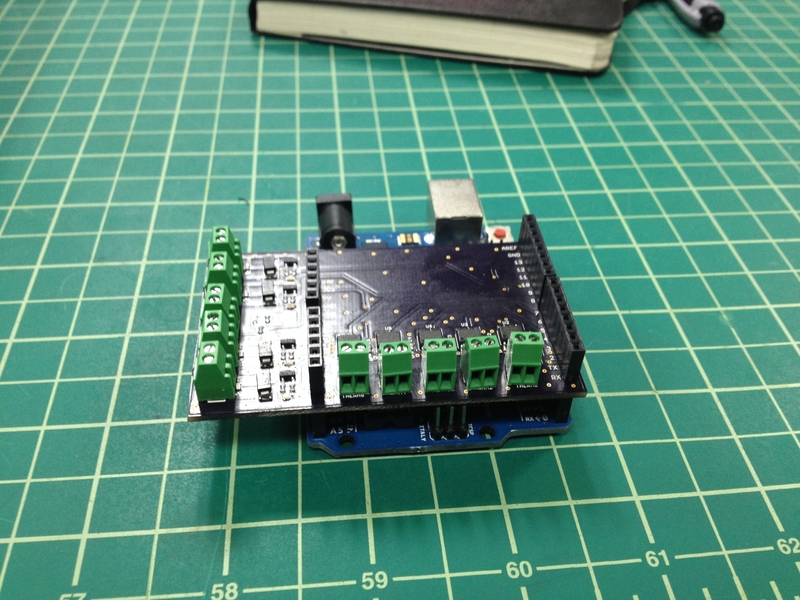
\includegraphics[width=0.8\linewidth]{ovenboard3-side.png}
\end{figure}
\end{frame}
%------------------------------------------------------

\begin{frame}
\frametitle{v3 Decisions}
\begin{figure}
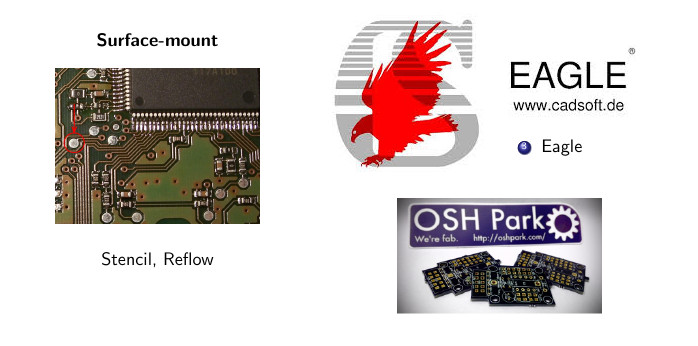
\includegraphics[width=1.0\linewidth]{decisions2.jpg}
\end{figure}
\end{frame}

%------------------------------------------------------

\begin{frame}
\frametitle{Using Digikey}
\begin{figure}
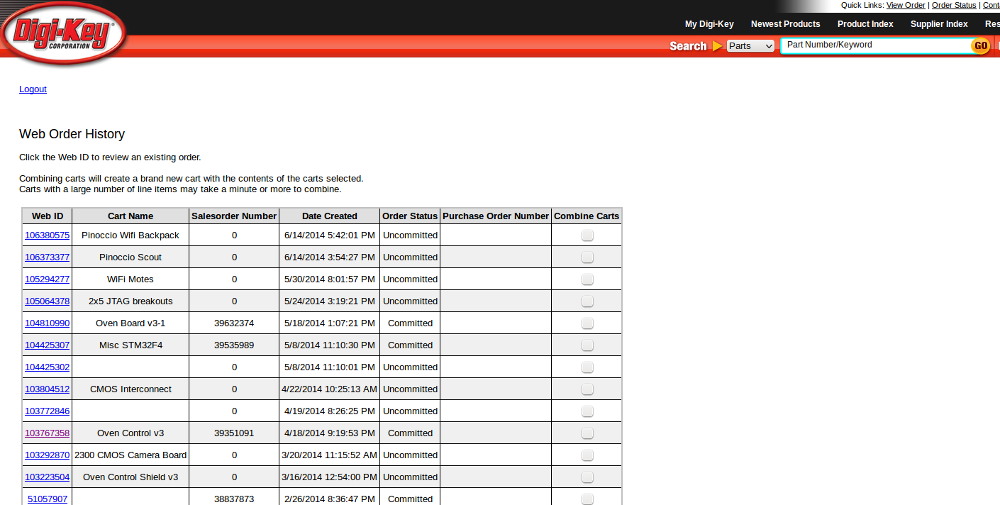
\includegraphics[width=1.0\linewidth]{digikey.png}
\end{figure}
\end{frame}

%------------------------------------------------------

\begin{frame}
\frametitle{Using Digikey}
\begin{figure}
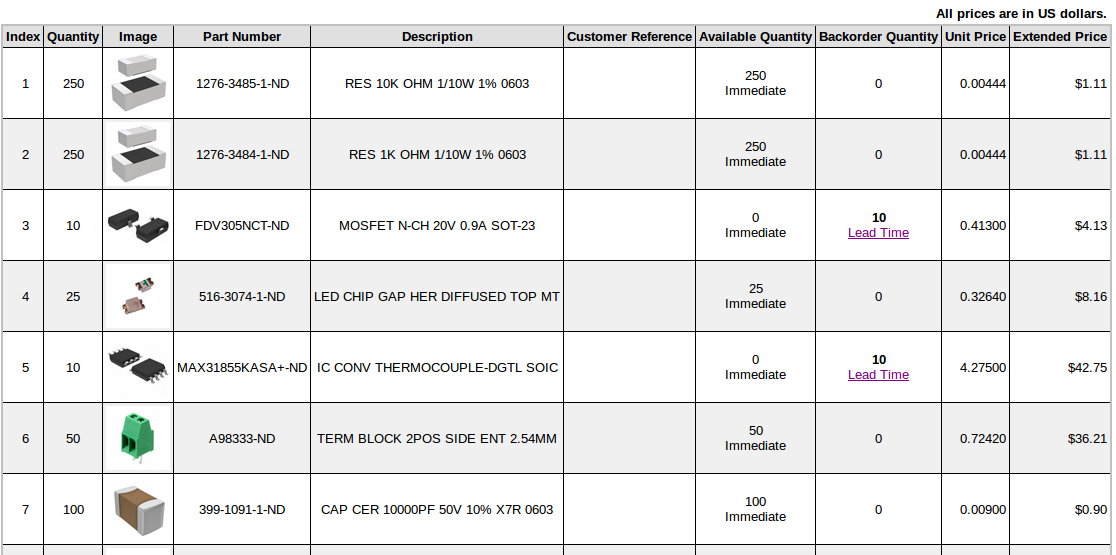
\includegraphics[width=1.0\linewidth]{parts.png}
\end{figure}
\end{frame}

%------------------------------------------------------

\begin{frame}
\frametitle{Working with Parts}
\begin{figure}
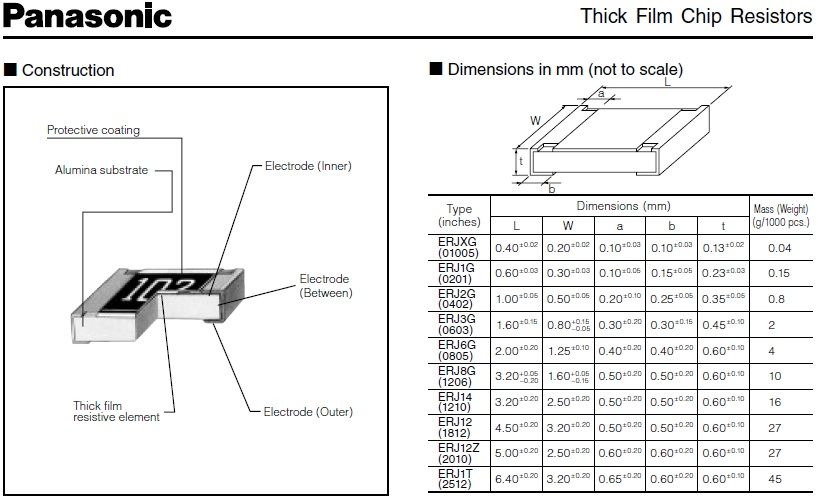
\includegraphics[width=1.0\linewidth]{panasonic.png}
\end{figure}
\end{frame}

%------------------------------------------------------

\begin{frame}
\frametitle{Working with Parts}
\begin{columns}[c] % The "c" option specifies centered vertical alignment while the "t" option is used for top vertical alignment

\column{.45\textwidth} % Right column and width
\begin{enumerate}
\item Temperature Coefficients
\item Storage (ESD, boxes) 
\item Heat and humidity 
\end{enumerate}

\column{.5\textwidth} % Right column and width
\begin{figure}
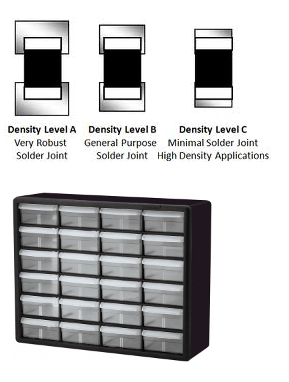
\includegraphics[width=1.0\linewidth]{resistors.png}
\end{figure}

\end{columns}
\end{frame}

%------------------------------------------------------

\begin{frame}
\frametitle{Update the circuit}
\begin{figure}
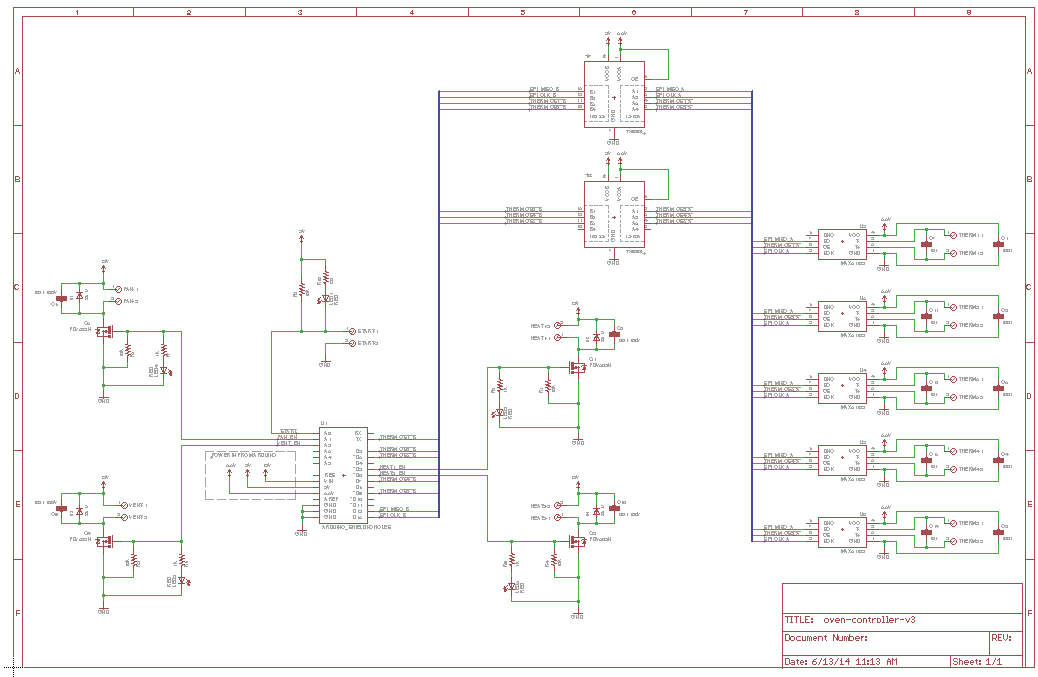
\includegraphics[width=1.0\linewidth]{v3sch.png}
\end{figure}
\end{frame}

%------------------------------------------------------

\begin{frame}
\frametitle{Update the circuit}
\begin{figure}
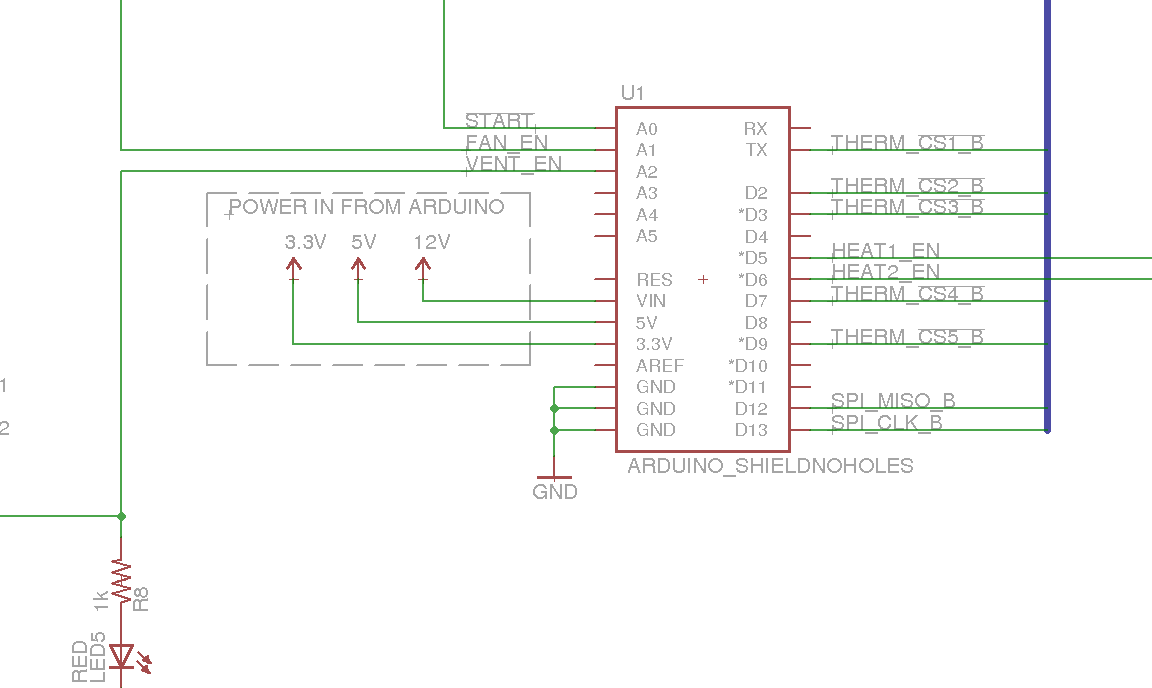
\includegraphics[width=1.0\linewidth]{sch-good.png}
\end{figure}
\end{frame}

%------------------------------------------------------

\begin{frame}
\frametitle{Example: FDV305N}
\begin{figure}
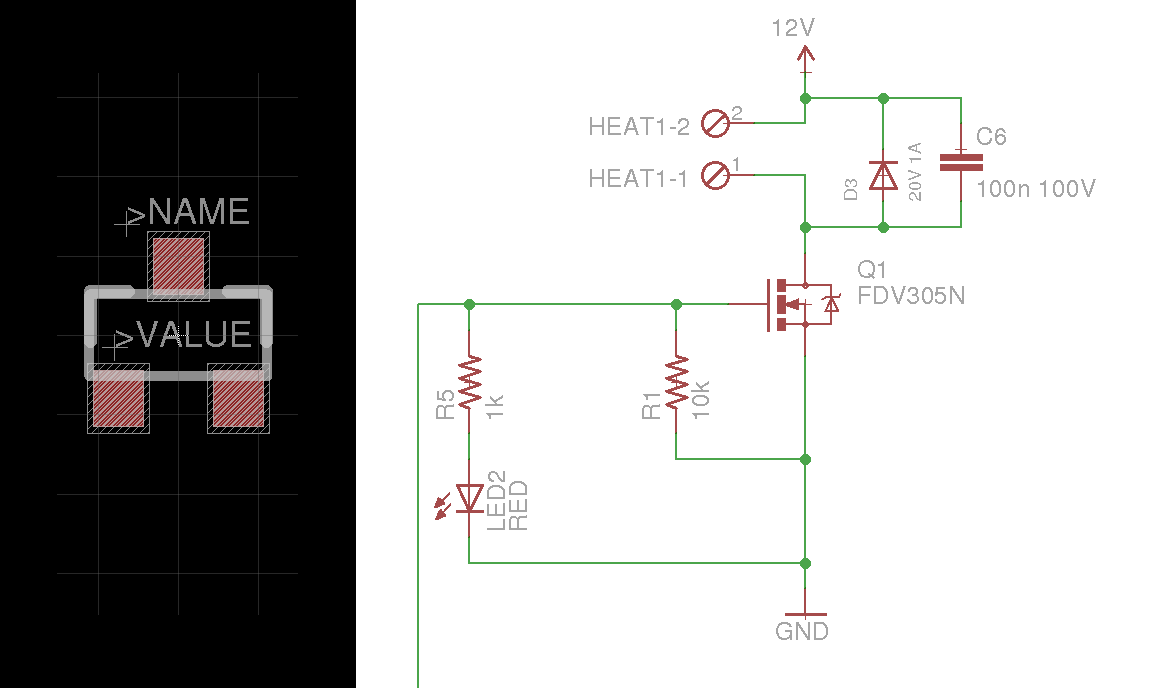
\includegraphics[width=1.0\linewidth]{fdv30n.png}
\end{figure}
\end{frame}

%------------------------------------------------------

\begin{frame}
\frametitle{The footprint is a lie}
\begin{figure}

\includegraphics[width=0.8\linewidth]{trustnoone.jpg}
\end{figure}
\end{frame}

%------------------------------------------------------

\begin{frame}
\frametitle{Land pattern}
\begin{figure}
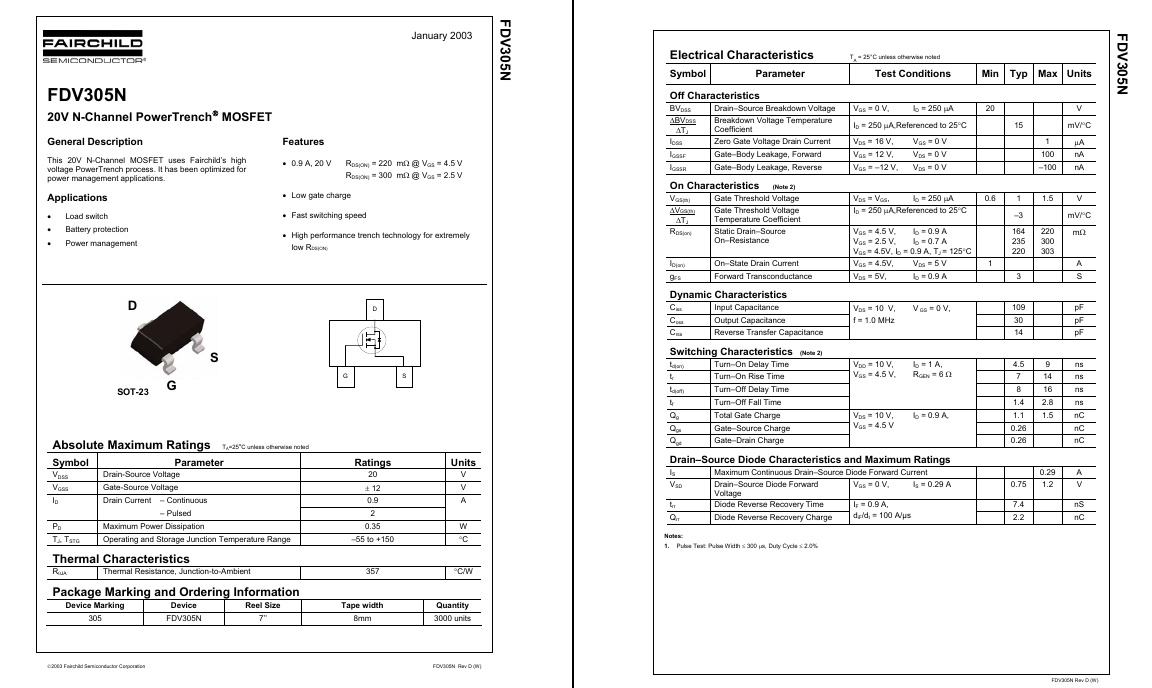
\includegraphics[width=1\linewidth]{datasheet.png}
\end{figure}
\end{frame}

%------------------------------------------------------

\begin{frame}
\frametitle{Land pattern}
\begin{figure}
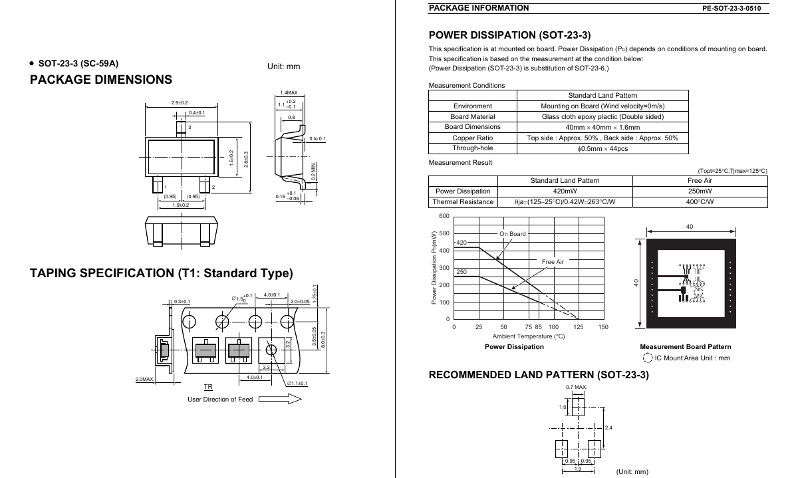
\includegraphics[width=1\linewidth]{sot23.png}
\end{figure}
\end{frame}

%------------------------------------------------------

\begin{frame}
\frametitle{Oven Board v3 Layout}
\begin{figure}
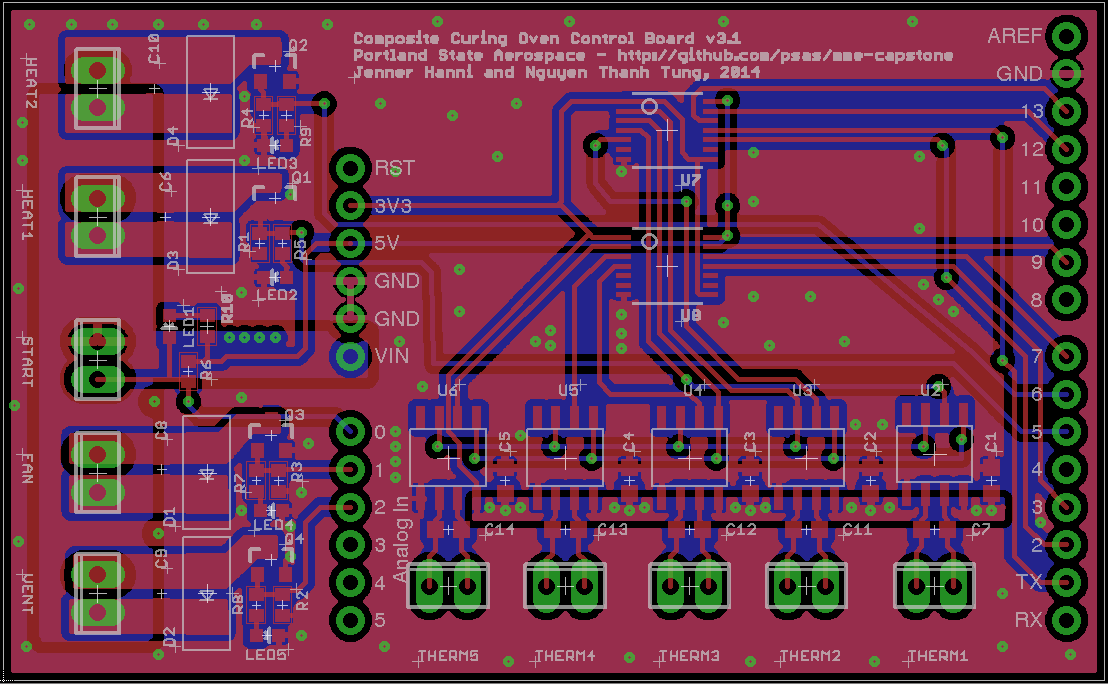
\includegraphics[width=1\linewidth]{v3board.png}
\end{figure}
\end{frame}

%------------------------------------------------------

\begin{frame}
\frametitle{Silkscreen}
\begin{figure}
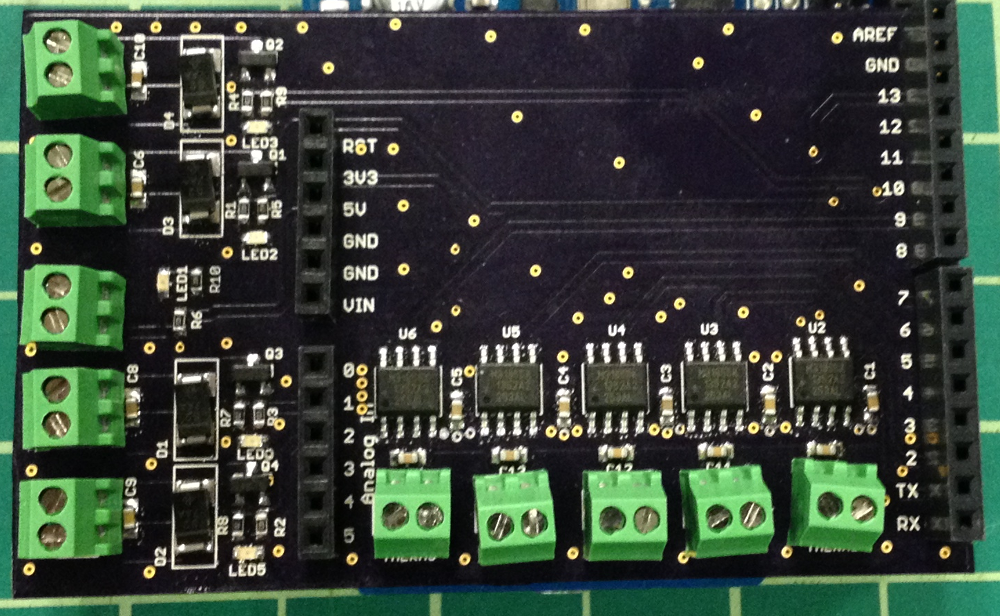
\includegraphics[width=1\linewidth]{silkscreen.png}
\end{figure}
\end{frame}

%------------------------------------------------------

\begin{frame}
\frametitle{Fab}
Order parts, then order the board. 
\end{frame}

%------------------------------------------------------

\begin{frame}
\frametitle{Assembly}
\begin{enumerate}
\item Make a stencil
\item Secure board in a jig
\item Place stencil on the jig
\item Spread solder paste
\item Remove the stencil
\item Prepare the parts
\item Place the surface mount parts
\item Place in the oven
\item Reflow the board
\item Test the board
\item Hand solder the through-hole parts
\end{enumerate}
\end{frame}

%------------------------------------------------------

\begin{frame}
\frametitle{Assembly: Paste Layer}
\begin{figure}
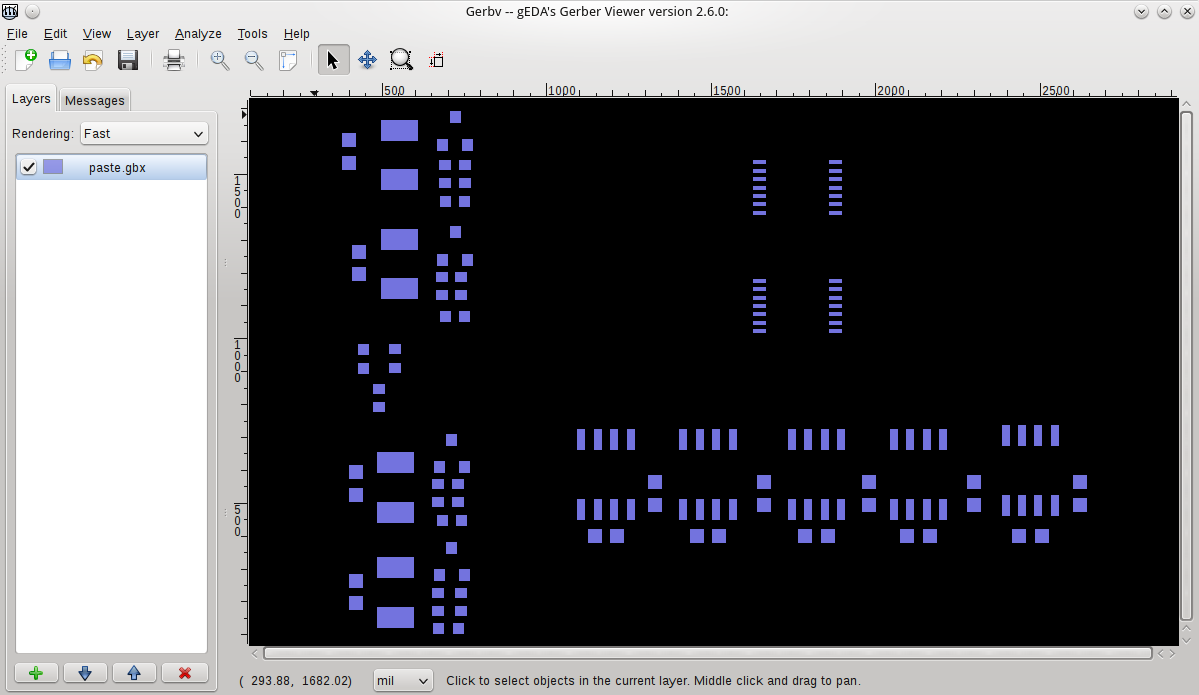
\includegraphics[width=0.9\linewidth]{soldermask-gerb.png}
\end{figure}
\end{frame}

%------------------------------------------------------

\begin{frame}
\frametitle{Assembly: Make a Stencil}
\begin{figure}
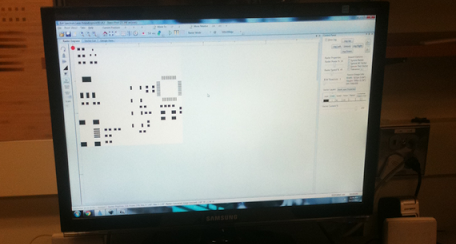
\includegraphics[width=0.9\linewidth]{assemble1.png}
\end{figure}
\end{frame}

%------------------------------------------------------

\begin{frame}
\frametitle{Assembly: Make a Stencil}
\begin{figure}
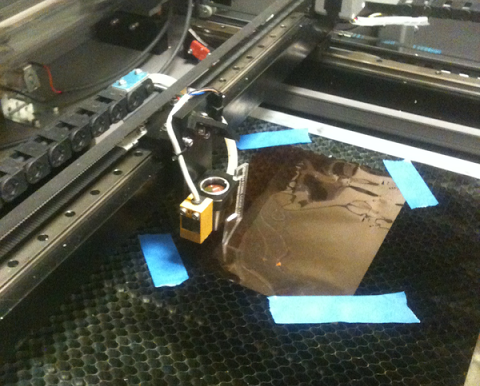
\includegraphics[width=0.8\linewidth]{assemble2.png}
\end{figure}
\end{frame}

%------------------------------------------------------

\begin{frame}
\frametitle{Assembly: Make a Stencil}
\begin{figure}
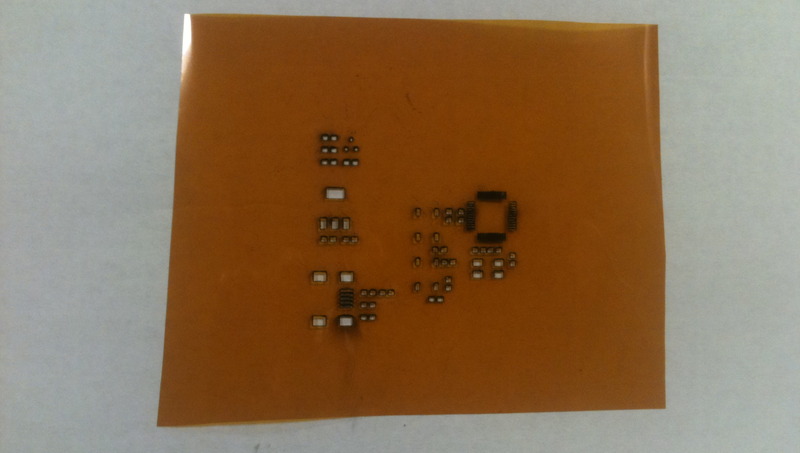
\includegraphics[width=0.9\linewidth]{assemble3.png}
\end{figure}
\end{frame}

%------------------------------------------------------

\begin{frame}
\frametitle{Assembly: Make a Stencil}
\begin{figure}
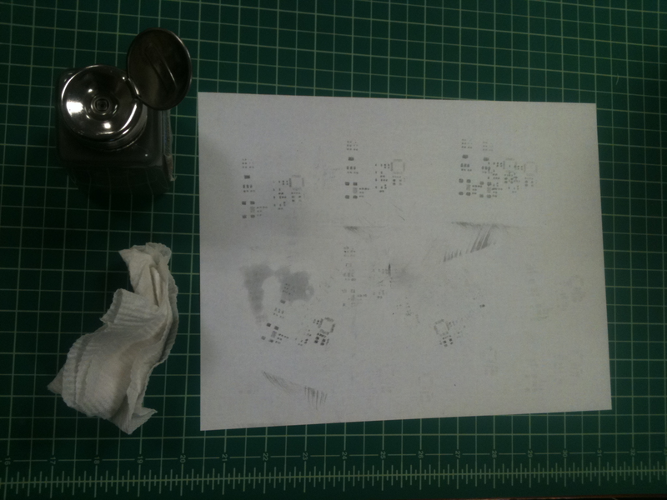
\includegraphics[width=0.8\linewidth]{assemble4.png}
\end{figure}
\end{frame}

%------------------------------------------------------

\begin{frame}
\frametitle{Assembly: Gather Parts}
\begin{figure}
\includegraphics[width=0.5\linewidth]{assemble5.png}
\end{figure}
\end{frame}

%------------------------------------------------------

\begin{frame}
\frametitle{Assembly: Prepare the Board}
\begin{figure}
\includegraphics[width=0.8\linewidth]{assemble6.png}
\end{figure}
\end{frame}

%------------------------------------------------------

\begin{frame}
\frametitle{Assembly: Secure the Board}
\begin{figure}
\includegraphics[width=0.8\linewidth]{assemble7.png}
\end{figure}
\end{frame}

%------------------------------------------------------

\begin{frame}
\frametitle{Assembly: Solder Paste}
\begin{figure}
\includegraphics[width=0.8\linewidth]{assemble10.png}
\end{figure}
\end{frame}

%------------------------------------------------------

\begin{frame}
\frametitle{Assembly: Prepare Parts}
\begin{figure}
\includegraphics[width=0.8\linewidth]{assemble9.png}
\end{figure}
\end{frame}

%------------------------------------------------------

\begin{frame}
\frametitle{Assembly: Place Parts and Reflow}
\begin{figure}
\includegraphics[width=0.8\linewidth]{assemble.png}
\end{figure}
\end{frame}

%------------------------------------------------------

\begin{frame}
\frametitle{Assembly: Place Parts and Reflow}
\begin{figure}
\includegraphics[width=0.8\linewidth]{assemble11.png}
\end{figure}
\end{frame}

%------------------------------------------------------

\begin{frame}
\frametitle{Assembly: Place Parts and Reflow}
\begin{figure}
\includegraphics[width=0.8\linewidth]{foxcar-built.png}
\end{figure}
\end{frame}

%------------------------------------------------------

\begin{frame}
\frametitle{Rework}
Wick, flux, solder sucker, vacuum, hot air gun. 
\begin{figure}
\includegraphics[width=0.8\linewidth]{rework.jpg}
\end{figure}
\end{frame}

%----------------------------------------------------------------------------------------
\section{Resources} 
\begin{frame}
\frametitle{All the things}
\begin{enumerate}
\item{IPC-A-610D: Acceptability of Electronics Assemblies}
\item{Henry Ott's Electromagnetic Compatibility Engineering}
\newline
\item{Sparkfun: http://learn.sparkfun.com}
\item{Adafruit: http://learn.adafruit.com}
\item{Oshpark: http://oshpark.com}
\item{PSU Electronics Prototyping Lab: http://psu-epl.github.io}
\newline
\item{Me: http://jennerhanni.net}
\item{My Github: http://github.com/wicker}
\end{enumerate}
\end{frame}
%------------------------------------------------------

\begin{frame}
\Huge{\centerline{The End}}
\end{frame}

%----------------------------------------------------------------------------------------

\end{document}
